\subsection{Voice User Simulator}
\label{sec:voice-user-simulator}

Voice interactions introduce challenges absent from text: the \textit{audio environment} degrades signals, and \textit{conversational dynamics} require real-time turn-taking decisions. Our simulator addresses these by generating realistic caller audio through a pipeline (Figure~\ref{fig:audio-pipeline}) combining text generation, speech synthesis, audio environment simulation, and conversational dynamics.

To isolate agent performance from transcription artifacts, the simulator receives the agent's transcript directly rather than transcribing agent speech.

\begin{figure}[ht]
\centering
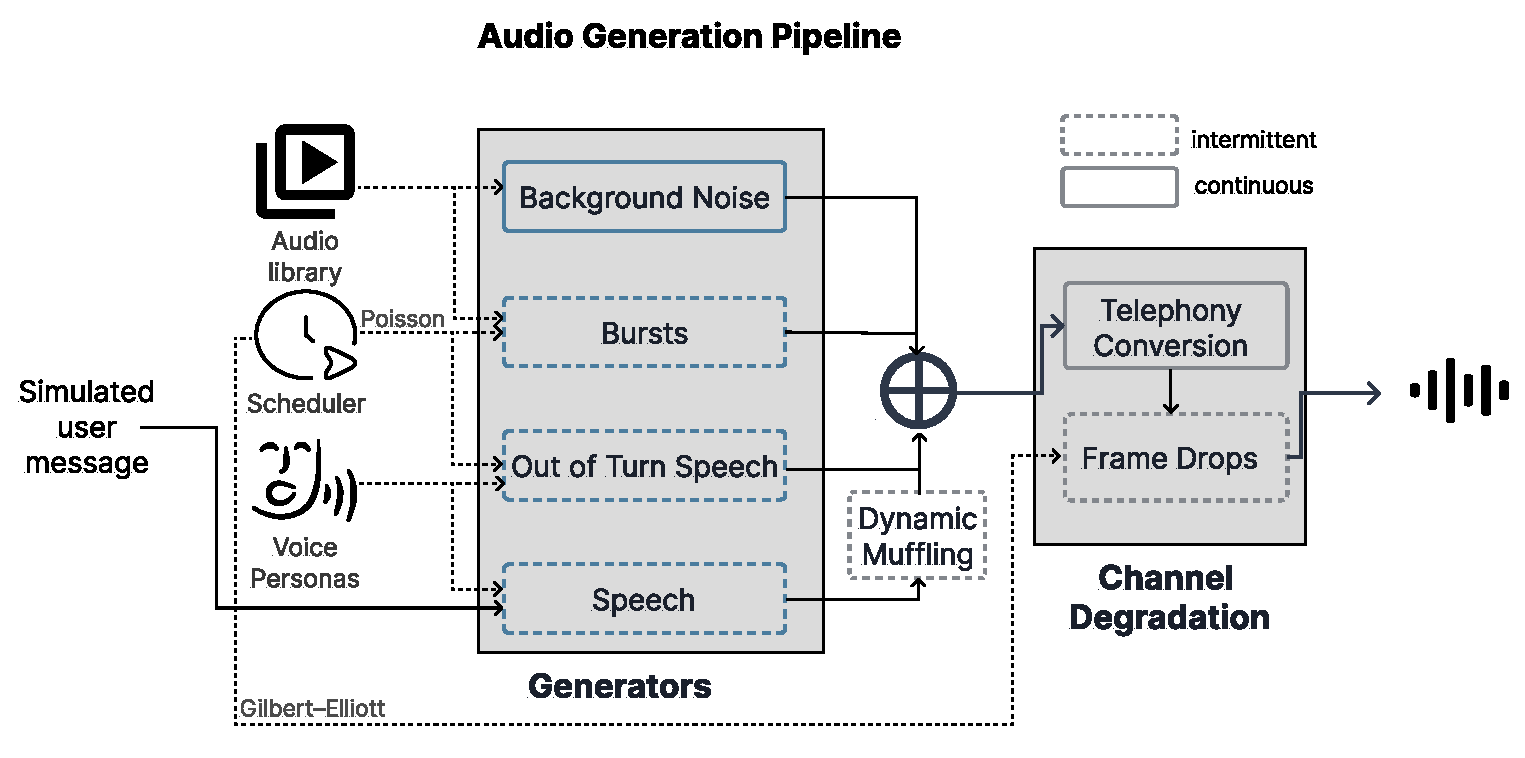
\includegraphics[width=\columnwidth]{figures/audio_pipeline.pdf}
\caption{Voice user simulator pipeline. Each tick, the simulator generates text, synthesizes speech with a persona, mixes in environmental audio, and applies telephony degradation to produce realistic caller audio.}
\label{fig:audio-pipeline}
\end{figure}

\paragraph{Speech Generation.} User simulator prompts produce natural spoken language: disfluencies and fillers (``um'', ``uh''), verbalized special characters (``at'' not ``@''), and terse responses. Generated text is synthesized using voice personas---each with a dedicated TTS voice and system prompt guiding speech style and prosody. We define seven personas spanning diverse accents and demographics (Appendix~\ref{app:personas}).

\paragraph{Audio Environment.} We simulate realistic telephony conditions by mixing synthesized speech with environmental audio: continuous background noise (chatter, traffic) and intermittent bursts (phone rings, dog barks) drawn from recorded samples. Out-of-turn speech---synthesized phrases like ``hold on'' and vocal tics like coughs and sneezes---simulates moments when callers are distracted. Effects degrade the signal: dynamic muffling simulates movement away from the microphone, telephony conversion applies G.711 $\mu$-law compression at 8kHz, and frame drops simulate packet loss. All streams are mixed to target signal-to-noise ratios relative to the primary speech. Parameters appear in Appendix~\ref{app:audio-effects}.

\paragraph{Turn-Taking Policy.} The simulator combines configurable threshold-based timing with LLM-driven decisions. For example, the user waits for a silence threshold (default 1s) before responding. During agent speech, an LLM periodically evaluates whether to interrupt based on conversation context. A separate LLM decides whether to backchannel (``mm-hmm''), and if the agent interrupts, the user yields after a configurable overlap duration. Full prompts appear in Appendix~\ref{app:turn-taking-prompts}; Table~\ref{tab:tick-example} illustrates these dynamics.
